\chapter{Hierarchical extensions of the LCA}\label{ch:hierarchical_sc}

%TODO: talk about hyvarninen... subspace ICA, topographic ICA, bubbles
\section{Introduction}\label{sec:ch3_intro}
We propose that a hierarchical model of natural scenes should produce a general representation of input data that spans all layers. The network should be able to model the causal structure of time-varying natural scenes. The bottom of the hierarchy should contain information about the details of the scene, and as one ascends the hierarchy, one should see a more general, abstract representation. Information should move up the hierarchy in the form of inference and down the hierarchy as expectations or priors. Resolving ambiguities at the top should be easier as there are more regularities and there is more context. This can then help inform inference in lower layers to resolve more difficult ambiguities about details of the scene. For this to occur, the network should perform causal inference in all layers simultaneously. The objective for the network should be to efficiently represent the independent underlying causes of incoming signal. While we will not be providing a single implementation of all of these ideas, we will review several important contributions and present novel architectures that put us closer to this goal.

\section{Hierarchical sparse coding models}\label{sec:ch3_related_models}
Broadly speaking, there have been many hierarchical unsupervised learning architectures in the literature. Here we will highlight work that is particularly relevant considering the aforementioned goals. Lee and Mumford \citeyearpar{lee2003hierarchical} propose a model that inspired what was described in the previous section. They simplify the model by forcing each layer to only receive input from the layers below and above, as in a Markov chain. Expectations are propagated down to alter priors for lower layers in a dynamic, context-sensitive manner. Feedback connections influence the inference process, causing a layer to converge on a solution that fits the expectations above and they use dynamic sampling algorithms to represent Bayesian inference. We believe a version that is true to the theory and uses sparse coding as a core computational framework is a promising direction for future research. Karklin and Lewicki \citeyearpar{karklin2003learning} propose a two-layer probabilistic model that is an extension of the ICA model. They start with learning a complete orthogonal basis with ICA, and then learn ``variance bases'' that model higher-order structure in images. Their network produces a hierarchical sparse distributed code of natural scenes, but instead of performing inference, they directly compute first layer activations using a feed-forward architecture. They are able to learn to represent higher-order structure such as elongated edges with a nonlinear (in the second layer) encoding process because the joint coefficient distribution is replaced with a hierarchical prior. As proposed, their model is not extendable to include additional layers, which we identify as a direction for improvement. Additionally, we are interested in extending the LCA network to include their probabilistic second layer. The variances learned in the second layer can then be used to guide LCA inference. Honghao Shan and colleagues propose a hierarchical model that alternates PCA-like and ICA transforms \parencite{shan2013efficient} and a second hierarchical model that recursively applies a pointwise nonlinear function of the ICA transform \citeyearpar{shan2007recursive}. These models learn visual features that resemble those found in the early stages of the primate vision system. In the first model they use PCA to reduce the input dimensionality and then overcomplete ICA \parencite{le2011ica} to learn higher order features from the PCA output. They show that when this process is repeated, their network continues to learn more interesting features. This model is a promising proof of concept for a framework that alternates dimensionality reduction and expansion to learn higher-order structure from natural images. In the second model they iteratively apply ICA with a pointwise nonlinear transform applied in between operations. The network learns features that qualitatively resemble higher-order features learned by other models. Cadieu and Olshausen \citeyearpar{cadieu2008learning} propose a two-layer sparse coding network that explicitly disentangles form and motion in the second layer when trained on video input. The first layer is a sparse coding model that is trained with complex valued dictionary elements. They then factorize the first layer output into two sets of second layer inputs that encode the time-derivative of the amplitude and phase components to explicitly separate form and motion, respectively. The second layer units also perform sparse coding on the logarithm of factorized quantities from the first layer. They demonstrate that form selective neurons develop invariance properties from the time-varying signal. We believe the use of time information from natural videos is a key component of learning a hierarchical representation of natural scenes that has high correspondence to what we see in biology. A convolutional LCA variant called the Deconvolutional Competitive Algorithm (DCA) is proposed in \parencite{paiton2015deconvolutional}. This model deconstructs images into a three-layer hierarchical code. The network performs inference in all three layers simultaneously, and all three layers compete to reconstruct the input. By configuring the strides and patch sizes appropriately, the network was designed such that each layer contributes a different degree of spatial detail to the reconstruction. The lowest layer reconstructed high spatial frequency, grayscale information while the highest layer reconstructed low spatial frequency and color information. However, the generative process is linear and therefore could be represented with a single dictionary. Ideally, we would like the generative process to be able to account for the non-linear structure in images. Additionally, the network does not learn to represent the higher-order \textit{structure} found in natural scenes, such as elongated edges. The sparse manifold transform, proposed by \parencite{chen2018sparse}, is an extendable hierarchical sparse coding network that models the underlying manifold structure of time-varying natural scenes (i.e. videos). The model combines dimensionality expansion using sparse coding and reduction using manifold embedding. The transform is also invertible via a non-linear generative process, such that linear translations in the embedded space result in non-linear transformations in the image space. The learned dimensionality reduction step can be thought of as an alternative to pooling operations commonly found in deep learning architectures.

In the following sections, we will propose two novel methods for extending the LCA to a hierarchical framework. The first is framed as a weakly-supervised machine learning network, while the second is an unsupervised model for learning invariant representations of natural scenes.

%TODO:
%\subsection{PCA dimensionality reduction to learn second layer units}
%Hyvarinen & Hoyer strong PCA work; my project implementing this with LCA
%Talks about LCA version of this
%https://docs.google.com/document/d/1RnKsawICMIf38o5eS8LmEdmkRHbOUxHzlJ5oLuu-bwo/edit


\section{Weakly-Supervised Feature Learning}\label{sec:ch3_weak_supervised_learning}
\subsection{Introduction}
We evolved a visual sense to allow us to understand the external causes of incident light.
The sensor modality is not designed to construct a veridical representation of the world \parencite{gollisch2010eye}.
Instead, it is designed to allow us to identify objects of significance and act upon them.
Our visual system is intimately connected with the statistics of light as it propagates through our natural world.
These statistics have been analyzed extensively by scientists exploring images and videos of natural scenes (see chapter 1). %TODO: Fix chapter refs
The sparse coding model represents an attempt to build on the knowledge gained from studying the statistics of natural scenes to better understand our visual system.
In the field of visual unsupervised machine learning, a cornucopia of models have been proposed to learn the statistics of natural scenes without human labels, or ``supervision'' (see \parencite{baldi2012autoencoders, bengio2012unsupervised, goodfellow2016deep} for reviews).
The unsupervised objective function of most of these models asks for a information-preserving latent representation of the inputs, often with an additional goal of compressing the signal through a bottleneck architecture.
However, when a reconstruction loss is combined with a family of constraints that include minimum entropy, maximum compression, and minimal energy expenditure, autoencoder models can exhibit interesting properties that are also found in biological vision systems.
In this chapter, we consider the LCA as an autoencoder.
Like an autoencoder, the LCA receives inputs, transforms them into a latent code, and produces reconstructions.
The LCA loss includes a term for information preservation, such that the input can be reconstructed from the encoding, as well as a constraint to minimize energy expenditure in the form of active neurons.
We are interested in understanding how useful the LCA can be for the machine learning field.
One way to assess this is to look at semi-supervised learning. Here the objective is the same as for supervised learning, where we want to associate images with some predetermined category label.
However, the catch is that many of the training images do not have ground truth labels assigned to them.
A fully supervised model would not be able to use these, and would suffer from limited training examples.
Here we show that the LCA can be used to improve semi-supervised learning results.
We also demonstrate how an alternate objective, such as labeling objects in the world, can be used in the LCA dynamics to modify inference and dictionary learning.

\subsection{Weakly-supervised learning}
%[https://docs.google.com/presentation/d/1Dy_Dy1uSnLC3FEWXczgdKGxSejRUYQmfHnwPtY5LA8Y/edit#slide=id.g12e96bb738_0_271]
%[https://docs.google.com/presentation/d/1CcFmB1AUIEWU_rKtIaiRM79QGMetjYhnjKfv58hDD8Y/edit#slide=id.g19049d0ee0_0_22]
%[https://docs.google.com/document/d/13IzufcIS9M9HTCKsQGPSWmCB7lbm4axBAVbGeEml-ks/edit?usp=sharing]
%[https://docs.google.com/presentation/d/1bW__4dYIlrrbiV55Y1WdKcI_jxYqCSPXVpQjnumrDfo/edit#slide=id.g13eab2f708_0_83 slide 11]

Human generated labels are extremely expensive to produce and often biased.
A learning paradigm that avoids this process is unsupervised learning, but it is not directly applicable to the machine learning task of assigning labels to data.
Weakly-supervised learning is a sub-field that aims to combine the benefits of unsupervised and supervised learning.
An ideal model should learn to categorize (e.g. cluster) data without ground-truth labels.
As we will demonstrate in chapter 4, sparse coding produces a code that is both descriptive and faithful to the image content. %TODO: Fix chapter refs
Here, we wish utilize the descriptive nature of the LCA by modifying it to utilize limited label information about an input scene.

\subsubsection{Features learned in unsupervised frameworks match those learned in supervised frameworks}
The Discriminative Recurrent Sparse Auto-Encoder (DrSAE, \cite{rolfe2013discriminative}) behaves similarly to sparse coding and has been shown to be successful at semi-supervised learning. Unlike LCA, the encoder, decoder, and lateral connectivity weights of DrSAE are unconstrained and trained independently. However, when trained on the MNIST dataset \parencite{lecun1998mnist}, the DrSAE learns weights that closely match what we impose for sparse coding. That is, the decoder weights have high correspondence to the transpose of the encoder weights and the lateral connectivity weights have high correspondence with the Gramian of the encoder weights. Additionally, when semi-supervised training is performed, the DrSAE learns an emergent hierarchical architecture. Figure \ref{fig:ch3_lenet_lca_drsae_weights} shows that the features learned by the unsupervised LCA and DrSAE models have a high degree of structural similarity to those learned by a supervised model \parencite{lecun1998gradient}. In general, supervised architectures require different types of regularization, such as dropout and weight decay, to learn structured weights.

% TODO: Add layer 1 from ReLU MLP?
\begin{figure}
    \centering
    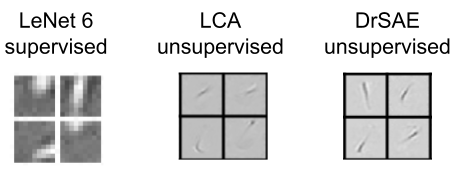
\includegraphics[width=0.5\textwidth]{figures/lenet_lca_drsae_weights.png}
    \caption{\textbf{Supervised and unsupervised learning produce similar weights.} The features learned from unsupervised training on MNIST using LCA \parencite{rozell2008sparse} and DrSAE \parencite{rolfe2013discriminative} have similar structure to those learned using the supervised LeNet model \parencite{lecun1998gradient}.}
    \label{fig:ch3_lenet_lca_drsae_weights}
\end{figure}

Given the success of the DrSAE model, we constructed a similar framework with the LCA. The LCA dynamics are derived from a principled energy function, so we were able to easily extend the framework by adding semi-supervised loss terms. In sparse coding the sparsity enforcing term is typically applied uniformly, penalizing all nodes. Instead of the prior limiting the total activation, we want the prior to encourage some nodes to be active based on expectations propagated down from higher layers. In our network, these higher layers are focused on grouping inputs into similar categories.

Our proposed network is capable of weakly-supervised learning, where only a small percentage of data examples have corresponding labels. We trained the models to categorize novel inputs using a heavily reduced set of labeled examples. Typical solutions to this problem utilize a combination of supervised and unsupervised learning objectives. The supervised objective aims to build an association between a given input and label, such that similar inputs receive the same label. The unsupervised learning objective aims to preserve a faithful representation of the input, such that the input data can be reconstructed directly from the network activations. In a typical scheme, the supervised objective is used when labels are available and the unsupervised objective is used when they are absent. In addition to these two classic objectives, we have added an additional unsupervised objective that encourages the network to confidently group the inputs into categories. This additional objective improves the network’s ability to categorize inputs, which is typically absent from unsupervised learning. The loss function minimizes the output entropy per image and maximizes it per batch. The intuition is that minimizing entropy per image will force the network to confidently place the image into a category, since the number of output nodes is small (e.g. 10 for MNIST). Maximizing the entropy across batches is intended to prevent the network from placing all images into a single category. It assumes that there is an approximately even distribution of classes in a given batch. We implemented this loss by adding a second layer on top of the LCA network that produced proposed categorical outputs. The network is trained using cross-entropy when there are labels or the combined entropy terms described earlier when there are not. Taking the derivative of this new cost with respect to a neuron's activation will give us a new update rule for sparse inference with the LCA.


\subsubsection{LCA with feedback}
A traditional deep network layer produces its output by filtering input data through a linear weight matrix and a nonlinear thresholding (i.e. activation) function.
The thresholded output is then passed to the next layer in the hierarchy.
Dimension-reducing nonlinearities, such as max-pooling, are often included between layers to increase network invariance for label-preserving variations.
They also prevent combinatorially increasing layer size with depth.
This process continues until, ultimately, a probability distribution over possible categories is produced as the final layer’s output.
For static data classification, such as image labeling, most deployed state-of-the-art networks are feedforward in that information strictly flows in one direction through the network.
Consequently, the layers themselves do not produce a dynamical response to the input.
In our alternative approach, the first layer of our network performs a dynamical non-linear computation on the input, which modifies the second layer outputs at each iteration.
The first layer is an LCA layer that incorporates lateral connectivity between neurons to enforce competition.
This results in a descriptive, distributed sparse code of the input data (see chapter 2 for details). %TODO: Fix chapter refs
The code is produced in a recurrent fashion, where the network dynamics evolve through time to a converged representation of the input.
Additionally, each LCA neuron receives input from the layer above that alters the dynamics in a context-dependent way.
The resulting network representation is hierarchical and faithful to the input, such that the data can be directly reconstructed from the first layer neuron activation values.
Within-layer competition and top-down feedback encourages the LCA to produce a descriptive code that is useful for image categorization.
The semi-supervised nature of the model will allow us to leverage raw data without the need for expensive human labeling.

\begin{figure}[h]
    \centering
    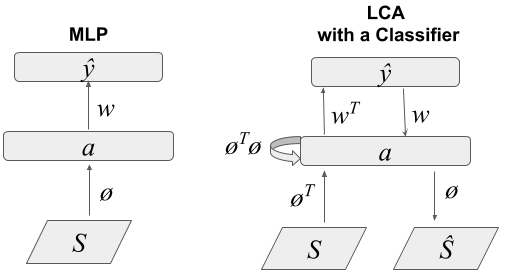
\includegraphics[width=0.5\textwidth]{figures/mlp_lcaf_architectures.png}
    \caption{\textbf{Training a classifier on LCA outputs.} We propose a two-layer LCA architecture that uses a semi-supervised objective in the second layer and we compare it against a standard 2-layer MLP architecture. In our experiments, we use different values for $\Phi$ in the MLP model: random, pre-trained to match that used for LCA, and trained using the traditional supervised learning method.}
    \label{fig:ch3_mlp_lcaf_architectures}
\end{figure}

For the LCA with feedback (LCAF) model, we will add an additional classification layer on top of the LCA model, as illustrated in figure \ref{fig:ch3_mlp_lcaf_architectures}. The network minimizes one of two different energy functions, depending on whether the input image has an associated label. In the case that there is a label, the energy function is the same as was used in equation \eqref{eq:ch2_sparse_energy}, with the addition of a cross-entropy term:

\begin{equation}\label{eq:ch3_lcaf_supervised_energy}
         E =
        \overbrace{ \tfrac{1}{2} \| s - \hat{s} \|_{2}^{2} }^\text{Preserve Information} +
        \overbrace{ \lambda \sum\limits_{i=1}^{M}C(a_{i}) }^\text{Limit Activations} -
        \overbrace{ \alpha \sum\limits_{j=1}^{K} y_{j}log(\hat{y_{j}})}^\text{Cross-Entropy Cost},
\end{equation}

\noindent where $K$ is the number of label categories, $\alpha$ is a tunable trade-off parameter, $y_{j}$ is a ground-truth one-hot label, and $\hat{y_{j}} = \frac{e^{-Wa_{j}}}{\sum_{n}e^{-Wa_{n}}}$ is the softmax output of the classification layer. When a label is not present, we swap out the cross-entropy cost with an entropy cost. We want our model to have high confidence (low entropy) per image and high entropy across batch (because we are assuming the categories are evenly distributed). We do this by defining two entropy terms. The first computes the entropy per image by summing across the neuron indices:

\begin{align}\label{eq:ch3_lcaf_q_dist}
\begin{split}
  Q_{b,k} &= \frac{e^{\hat{y}_{b,k}}}{\sum\limits_{j=1}^{K}e^{\hat{y}_{b,j}}} \\
  H^{\text{neuron}}_{b} &= -\sum\limits_{k}^{K}Q_{b,k}\log Q_{b,k}.
 \end{split}
\end{align}

The second term computes the batch entropy by summing across the batch dimension:

\begin{align}\label{eq:ch3_lcaf_p_dist}
\begin{split}
  P_{b,k} &= \frac{e^{\hat{y}_{b,k}}}{\sum\limits_{j=1}^{B} e^{\hat{y}_{j,k}}} \\
  H^{\text{batch}}_{k} &= -\sum\limits_{b=1}^{B}P_{b,k}\log P_{b,k},
 \end{split}
\end{align}

\noindent where $B$ is the batch size and $K$ is the number of softmax outputs. Now we can combine these terms for our unsupervised entropy loss:

\begin{equation}\label{eq:ch3_lcaf_unsupervised_energy}
         E =
        \overbrace{ \tfrac{1}{2} \| s - \hat{s} \|_{2}^{2} }^\text{Preserve Information} +
        \overbrace{ \lambda \sum\limits_{i=1}^{M}C(a_{i}) }^\text{Limit Activations} +
        \overbrace{ \alpha_{1} \sum\limits_{b=1}^{B} H^{\text{neuron}}_{b} - \alpha_{2} \sum\limits_{k=1}^{K}H^{\text{batch}}_{k}}^\text{Entropy Cost},
\end{equation}

\noindent where $\alpha_{1}$ and $\alpha_{2}$ are tunable loss trade-off parameters. Our LCA inference equation follows the same derivation from equation \eqref{eq:ch2_lca_deda_simple}, with an added term computed from the derivative of the entropy or cross-entropy costs with respect to the activity vector, $a$.

%TODO: add lca update rule / (cross) entropy derivatives from lab book
%(https://docs.google.com/presentation/d/1Dy_Dy1uSnLC3FEWXczgdKGxSejRUYQmfHnwPtY5LA8Y/edit#slide=id.g12e96bb738_0_211 for cross-entropy) 

\subsection{Experiments on MNIST dataset}
Our fist experiment is to verify that the classifier is able to train using sparse codes as input. The following table gives the MNIST test accuracy using a fully supervised label set. The LCA model was pre-trained on MNIST without labels and then a single layer perceptron (SLP) classifier was trained on the activity vector, $a$. Our results indicate that the LCA+SLP network out performs the MLP network.

%TODO: Cross-validate these scores
\begin{table}[]
\begin{tabular}{lllll}
 & \textbf{MLP} & \textbf{\begin{tabular}[c]{@{}l@{}}MLP with\\ random $\Phi$\end{tabular}} & \textbf{\begin{tabular}[c]{@{}l@{}}MLP with\\ LCA $\Phi$\end{tabular}} & \textbf{\begin{tabular}[c]{@{}l@{}}LCA with\\ classifier\end{tabular}} \\ \cline{2-5} 
\multicolumn{1}{l|}{\textbf{Test Error}} & \multicolumn{1}{l|}{411} & \multicolumn{1}{l|}{2979} & \multicolumn{1}{l|}{1723} & \multicolumn{1}{l|}{331} \\ \cline{2-5} 
\multicolumn{1}{l|}{\textbf{Test Accuracy}} & \multicolumn{1}{l|}{95.89\%} & \multicolumn{1}{l|}{70.21\%} & \multicolumn{1}{l|}{82.77\%} & \multicolumn{1}{l|}{96.69\%} \\ \cline{2-5} 
\end{tabular}
\caption{\textbf{LCA helps with MNIST classification.} This table shows that a single layer classifier trained on LCA encodings of the MNIST digit dataset outperforms a two layer classifier trained directly on MNIST pixels. The first column is the results for a two-layer classically trained MLP. The second is the same, except that the first layer weights were frozen with random initialization. The third had the first layer weights frozen to those that were trained with LCA, but did not utilize sparse inference. The final column is the results for a single-layer classifier trained on the LCA activations.}
\label{tab:ch3_mnist_accuracy}
\end{table}

Next we modified the MNIST dataset such that a varying percentage of the labels are removed to test our network’s ability to generalize and label unseen digit images. In table \ref{tab:ch3_restricted_mnist_accuracy}, we show that adding supervised cross-entropy feedback to sparse inference had little effect in the limited label regime. However, combining the supervised cross-entropy feedback with the unsupervised entropy feedback resulted in an improved score with very few labeled examples. These scores were not cross-validated, and therefore we cannot assign confidence intervals to the accuracy reported. The error rates found from previous studies were 0.1\%, 1\%, and 5\% for 50000, 100, and 20 labeled examples respectively \parencite{rasmus2015semi}. We expect that our error rates would be close to those previously reported, as they largely stem from variation in the training and validation sampling.

\begin{table}[]
\begin{tabular}{llll}
\multicolumn{1}{c}{\textbf{\begin{tabular}[c]{@{}c@{}}Number of labeled\\ training examples\end{tabular}}} & \multicolumn{1}{c}{\textbf{LCA}} & \multicolumn{1}{c}{\textbf{\begin{tabular}[c]{@{}c@{}}LCAF\\ sup only\end{tabular}}} & \multicolumn{1}{c}{\textbf{\begin{tabular}[c]{@{}c@{}}LCAF\\ sup \& unsup\end{tabular}}} \\ \cline{2-4} 
\multicolumn{1}{l|}{\textbf{50,000}} & \multicolumn{1}{l|}{96\%} & \multicolumn{1}{l|}{96\%} & \multicolumn{1}{l|}{96\%} \\ \cline{2-4} 
\multicolumn{1}{l|}{\textbf{100}} & \multicolumn{1}{l|}{68\%} & \multicolumn{1}{l|}{67\%} & \multicolumn{1}{l|}{65\%} \\ \cline{2-4} 
\multicolumn{1}{l|}{\textbf{20}} & \multicolumn{1}{l|}{33\%} & \multicolumn{1}{l|}{33\%} & \multicolumn{1}{l|}{38\%} \\ \cline{2-4} 
\end{tabular}
\caption{\textbf{Feedback helps with MNIST classification.} We compare the LCAF model against two variants: One with strictly supervised feedback (middle column) and another with supervised and unsupervised feedback (right column). Although the feedback does not appear to help when there are a large number of labeled examples, it does show a positive effect when the number of labeled examples is restricted.}
\label{tab:ch3_restricted_mnist_accuracy}
\end{table}

To test whether the unsupervised feedback term produces a meaningful signal for inference, we measured the distances among sparse codes produced without feedback, with supervised feedback, and with unsupervised feedback. Figure \ref{fig:ch3_feedback_code_distances} shows that the Hamming distance between codes produced with either form of feedback is smaller than the distance from a code produced with feedback to one produced without feedback. Here we measure Hamming distance as the number of flipped bits between binarized vectors where a 1 indicates that a neuron's membrane potential, $u$, crossed threshold (i.e. went from active to inactive or vice versa) and a 0 indicates otherwise. This tells us that the feedback itself changes the code produced, and also that the unsupervised feedback produces a code that is similar to the supervised feedback code. This suggests that the unsupervised feedback is a good proxy for the supervised signal.

\begin{figure}
    \centering
    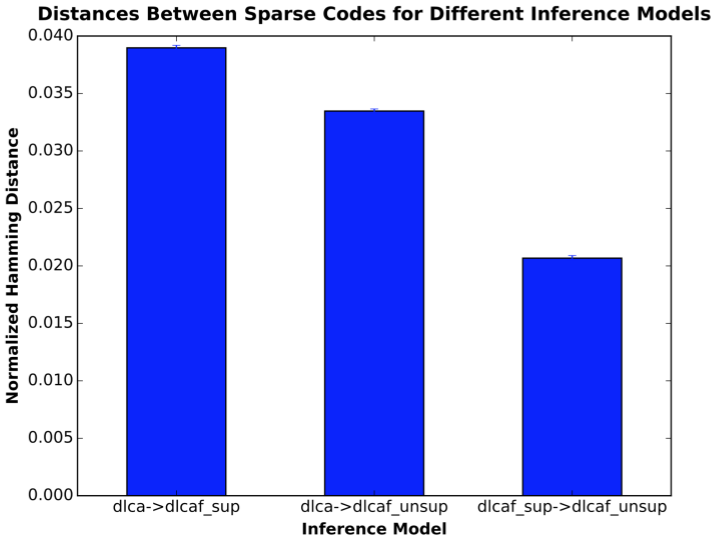
\includegraphics[width=0.5\textwidth]{figures/feedback_code_distances.png}
    \caption{\textbf{Unsupervised feedback during LCA inference produces similar codes to supervised feedback.} We measure the number of neurons that crossed their activation threshold (from active to inactive or vice versa) in terms of a Hamming distance. The distances between the codes produced without feedback and with either form of feedback (left two bars) are larger than the distance between the codes produced with supervised and unsupervised feedback (right bar). This tells us that the unsupervised entropy feedback produces a meaningful signal that is similar to that produced by supervised cross-entropy feedback. The bars height indicates mean hamming distance for 100 images and error bars indicate standard error of the mean.}
    \label{fig:ch3_feedback_code_distances}
\end{figure}

We also tested the weights learned with and without feedback during inference. In this experiment, the dictionary update rule is the same as was described in equation \eqref{eq:ch2_phi_update}, but the sparse inference process was modified. Figure \ref{fig:ch3_feedback_nofeedback_features} shows that the feedback process influences the first layer weights, which learned to produce more prototypical digits. Additionally, the first layer neurons that are most strongly connected to a specific second layer classification neuron have a higher degree of correspondence to the classification category when feedback was used during inference.

\begin{figure}
    \centering
    \begin{subfigure}[b]{0.9\textwidth}
        \centering
        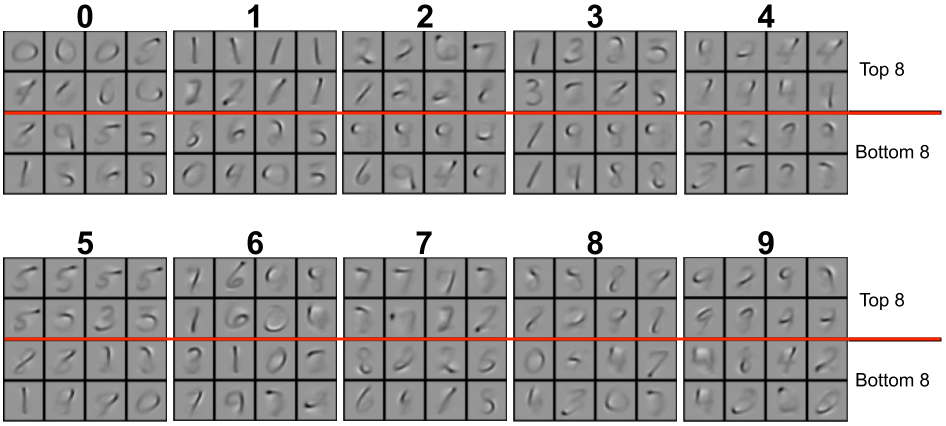
\includegraphics[width=\textwidth]{figures/lca_nofeedback_classifier_features.png}
        \caption{Without feedback}
        \label{fig:ch3_nofeedback_features}
    \end{subfigure}
    \begin{subfigure}[b]{0.9\textwidth}
        \centering
        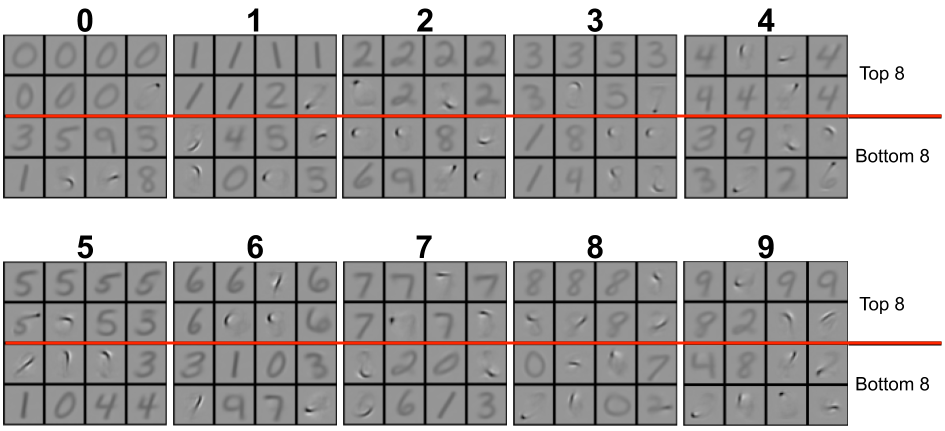
\includegraphics[width=\textwidth]{figures/lca_feedback_classifier_features.png}
        \caption{With supervised feedback}
        \label{fig:ch3_feedback_features}
    \end{subfigure}
    \caption{\textbf{Feedback influences weight gradients for the LCAF network.} The subfigures show the basis functions, $\Phi$, for the top and bottom strongest connected first layer neurons to each classification output neuron. (a) Inference was performed with supervised feedback. (b) Inference was performed without feedback. Each 4x4 grid corresponds to a particular classification label. Images above the red line are the basis functions for the 8 neurons that are most strongly connected to the given classification neuron and below the red line are the bottom 8. The basis functions themselves change with feedback, and the structure of the top connected basis functions is better matched to the digit label when feedback is used.}
    \label{fig:ch3_feedback_nofeedback_features}
\end{figure}

\subsection{Conclusion}
We proposed a two-layer LCA network extension that uses semi-supervised loss signals to direct sparse inference. We showed that the feedback signal influences the weights learned and improves classifications accuracy when there is a restricted set of labels. In the following section, we propose a alternative two-layer LCA network that is completely unsupervised. Combining the ideas from these two sections is a current area of research.

\section{Subspace LCA}\label{sec:ch3_subspace_lca}
\subsection{Introduction}
We describe an extension to the LCA model that produces invariant representations of its inputs. The model is similar to Independent Subspace Analysis \parencite{hyvarinen2000emergence}, but differs in several key ways. First, the LCA model allows for the first layer representation to be overcomplete, which improves efficiency \parencite{lewicki2000learning}. Second, the first layer encoding process is non-linear, which further improves efficiency as well as selectivity (see section \ref{sec:ch4_selectivity_efficiency}).

\subsection{Model description}
The subspace LCA follows a similar derivation to the LCA (section \ref{sec:ch2_lca}). Like the LCA, it learns a set of weights to efficiently describe natural signals, although in this variant we constrain the weights to be grouped. We set the number of neurons in a group as a hyper-parameter. We start with the same generative framework as in sparse coding (equation \ref{eq:ch2_sparse_generative_model}). We will constrain our activations (and therefore weights) to non-overlapping groups that have an amplitude, $\sigma$:

\begin{align}\label{eq:ch3_a_decomp}
\begin{split}
  \sigma_{i} = ||a_{i}||_{2} = \sqrt{\sum_{j\in L}a^{2}_{ij}},
\end{split}
\end{align}

\noindent where $i$ indexes the group and $j \in L$ indexes the neuron within the group. The group amplitude is equivalent for many combinations of $a_{j \in L}$. Each of these equal combinations can be thought of as a direction of a vector in the activity space. We define this as a unit-length direction vector, $z$, that has the same number of elements as our activity vector:

\begin{align}\label{eq:ch3_z_def}
\begin{split}
  z_{ij} = \frac{a_{ij}}{\sigma_{i}}.
\end{split}
\end{align}

We can now define a new energy function in these terms. We also add a regularization term that pressures the within-group weights to be orthogonal, which prevents the pathological solution of within-group neurons learning to have identical weights. This regularization term will also reduce competition between neurons within groups, which is scaled by the inner product between neighboring neurons' weight vectors.

\begin{equation}\label{eq:ch3_subspace_lca_energy}
    E = \frac{1}{2}\sum_{p}\left[s_{p} - \sum_{ij}\sigma_{i}z_{ij}\Phi_{ijp}\right]^{2} + \lambda \sum_{i}\sigma_{i} + \alpha \sum_{ij}\left|\sum_{p} \Phi_{ijp}\Phi_{ijp} - \mathbf{I}_{L} \right|,
\end{equation}

\noindent where $\alpha$ is a trade-off multiplier, $\mathbf{I}_{L}$ is the $L \times L$ identity matrix, and $L$ is the number of neurons in a group. Following the LCA derivation in section \ref{sec:ch2_lca}, we will next take the derivative of the energy with respect to neuron $k$'s activity:

\begin{equation}\label{eq:ch3_subspace_deda}
    -\frac{\partial E}{\partial a_{ik}} = \sum_{p}s_{p}\phi_{ikp} - \sum_{lm}G_{iklm}a_{lm} - \lambda \frac{\partial ||a_{i}||^{2}}{\partial a_{ik}}.
\end{equation}

We can rewrite the last term in the above equation as our direction vector:

\begin{align}\label{eq:ch3_subspace_deda_to_z}
\begin{split}
    \frac{\partial ||a_{i}||^{2}}{\partial a_{ik}} &= \frac{1}{2}\left(\sigma_{i}^{2}\right)^{-\tfrac{1}{2}}2a_{ik}\\
    &= \frac{a_{ik}}{\sigma_{i}}\\
    &= z_{ik}.
\end{split}
\end{align}

In parody with the LCA derivation, we group the self inhibition terms:

\begin{align}\label{eq:ch3_f_of_a}
\begin{split}
    f_{\lambda}(a_{ik}) &= a_{ik} + \lambda z_{ik}\\
    &= \left(\sigma_{i}+\lambda\right) z_{ik}\\
    &= a_{ik}(1 + \frac{\lambda}{\sigma_{i}}).
\end{split}
\end{align}

We again assign our membrane potential, $u$ as a function of $a$:

\begin{equation}\label{eq:ch3_u_def}
  u_{ik} = f_{\lambda}(a_{ik}) = (\sigma_{i} + \lambda)z_{ik},
\end{equation}

which also gives us an alternative definition for the neuron angle, $z$:

\begin{equation}\label{eq:ch3_z_u_def}
   z_{ik} = \frac{u_{ik}}{\sigma_{i} + \lambda} = \frac{u_{ik}}{||a_{i}||_{2} + \lambda}.
\end{equation}

The resulting membrane update rule is nearly identical to equation \ref{eq:ch2_u_dot_full}, except that the lateral competition term includes group assignments:

\begin{equation}\label{eq:ch3_subspace_u_dot_def}
   \tau \dot{u_{ik}} - u_{ik} = \sum_{p}s_{p}\phi_{ikp} \sum_{lm \ne ik}G_{iklm}a_{lm}.
\end{equation}

Finally, we define the output amplitude in terms of the group threshold:

\begin{equation}\label{eq:ch3_subspace_threshold_func}
    a_{ik} = T_{\lambda}(\sigma_{i}) = \left\{
    \begin{aligned}
        0,\;\; & \sigma_{i}\; \leq\; \lambda \\
        (\sigma_{i}-\lambda)z_{ik},\;\; &\sigma_{i}\; >\; \lambda.
    \end{aligned}
    \right.
\end{equation}

This tells us that all within-group neurons become active when the group amplitude surpasses the threshold, $\lambda$. Figure \ref{fig:ch3_subspace_lca_graph} shows a diagram of the group model.

\begin{figure}[h]
    \centering
    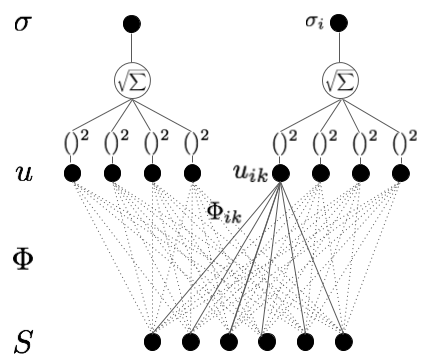
\includegraphics[width=0.4\textwidth]{figures/subspace_lca_graph.png}
    \caption{\textbf{Subspace LCA}. Neurons are grouped such that they learn subspaces of co-active units. Once a group amplitude passes the threshold, all neurons in the group produce an output activity that is modulated by the direction vector, $z$.}
    \label{fig:ch3_subspace_lca_graph}
\end{figure}

\subsection{Features learned}
When trained on natural images, the weights learn to tile orientations, spatial frequencies, and positions just like regular LCA. They also learn to have within-group similarities, such as equal orientation or position.

\begin{figure}[h]
    \centering
    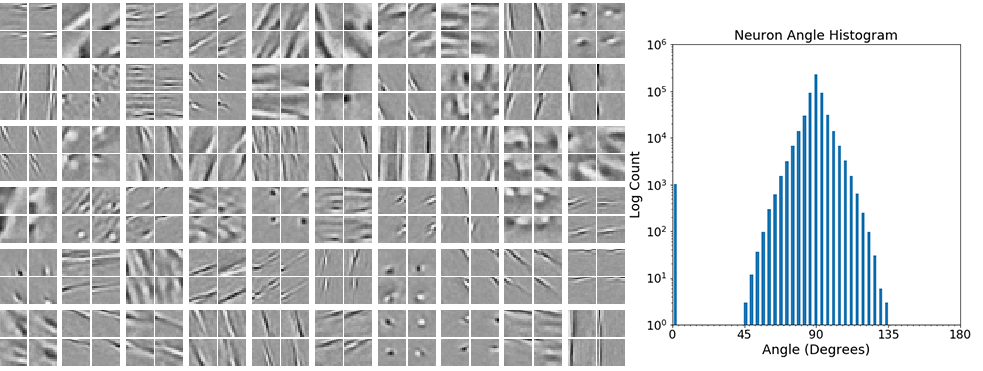
\includegraphics[width=\textwidth]{figures/subspace_lca_vh_features.png}
    \caption{\textbf{Natural image features learned with subspace LCA}. The left plot shows that subspace LCA learns features that have similar properties within group, but are different across groups. The right plot shows that the basis function angle histogram is very similar to that learned with the LCA.}
    \label{fig:ch3_subspace_lca_vh_features}
\end{figure}

Interestingly, we show in figure \ref{fig:ch3_subspace_lca_mnist_features} that the group structure naturally separates digit classes when the model is trained without supervised labels on the MNIST dataset. We believe this shows promise to use this model in a semi-supervised framework similar to that described in section \ref{sec:ch3_weak_supervised_learning}.

\begin{figure}[h]
    \centering
    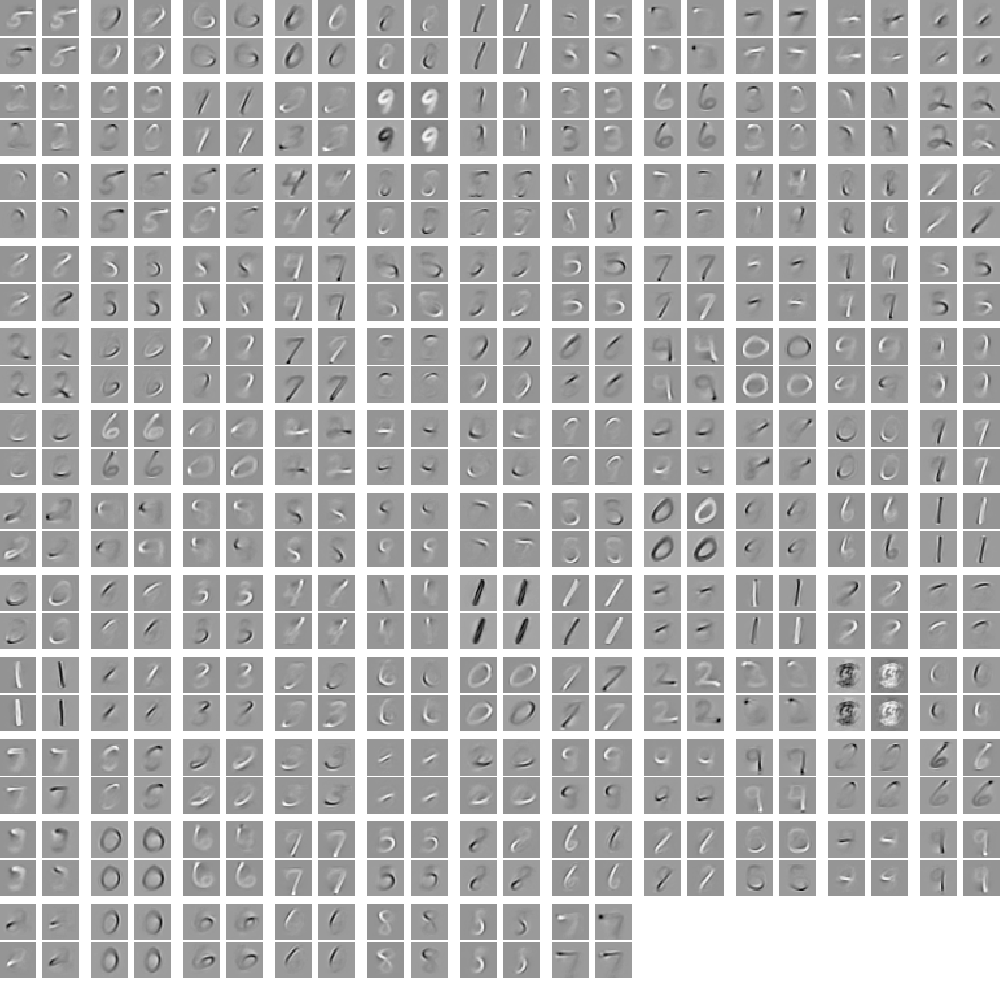
\includegraphics[width=0.8\textwidth]{figures/subspace_lca_mnist_features.png}
    \caption{\textbf{MNIST features learned with subspace LCA}. The features learned with this model natural separate into digit categories, indicating that it might be a simple operation to assign images labels from the group amplitude representations.}
    \label{fig:ch3_subspace_lca_mnist_features}
\end{figure}

\section{Conclusion}\label{sec:ch3_conclusion}
Hierarchical structure is found throughout cortex, but the underlying computation being performed by this structure is largely unknown. We propose that Bayesian efficient coding models can be extended into a hierarchical framework and in section \ref{sec:ch3_related_models} we provided several supporting examples from the literature. In section \ref{sec:ch3_weak_supervised_learning}, we proposed a hierarchical extension whereby a classifier is trained on the outputs of the LCA. Our semi-supervised network learns a hierarchical representation of visual data with or without corresponding labels. Instead of a narrowly specified task, the primary objective of our model is to construct a general, hierarchical and efficient code of the data that can be applied to a myriad of different tasks. This section showcased a promising research direction of using supervised and unsupervised entropy signals to direct LCA inference. Future work includes investigating further how feedback influences inference and learning, how the depth of the classifier influences inference and learning, as well as making comparisons to alternative methods.

In section \ref{sec:ch3_subspace_lca}, we demonstrate a novel extension of the LCA that learns statistical dependencies of sparse codes by grouping co-active elements into subspaces. Future work includes drawing comparisons to the Independent Subspace Analysis (ISA - \cite{hyvarinen2000emergence}) and extending the model to a topographic version. Also, we believe this formulation can be extended to include ideas from dynamic routing \parencite{olshausen1993neurobiological}, where the $z$ variables ``steer'' the output representation.